\section{Conclusion et recommandations}
\markboth{6. Conclusion et recommandations}{}

\subsection{Récapitulatif des décisions}

\begin{table}[H]
\centering
\small
\begin{tabularx}{\linewidth}{@{}L{4.2cm}XL{2.6cm}@{}}
\toprule
\textbf{Décision} & \textbf{Fondement} & \textbf{Nature} \\
\midrule
Supprimer les variables en fuite & Un utilisateur capable de les renseigner n'a pas besoin du modèle & Structurante \\
Accompagner toute estimation d'une fourchette & Un nombre seul est lu comme une mesure & Structurante \\
Fixer le niveau de confiance à 75\,\% & Au-delà, la fourchette cesse d'être exploitable & Arbitrage produit \\
Écarter TabPFN & Licence \emph{et} 101 fois l'énergie pour un gain dans le bruit & Sur mesure \\
Écarter la régression quantile conformalisée & Gain de couverture conditionnelle dans le bruit & Sur mesure \\
Écarter \code{ParkingRatio} & Confirme un arbitrage de la solution auditée & Sur mesure \\
Basculer vers Gradio & Seul chemin gratuit après changement des conditions de l'hébergeur & Contrainte subie \\
Ne pas écrire de \code{Dockerfile} & Non déployé, il aurait constitué une dette & Arbitrage assumé \\
Ne pas superviser la dérive & Coût de maintenance $>$ bénéfice à cette échelle & Arbitrage assumé \\
Versionner les artefacts avec le code & 2,1~Mo : un téléchargement n'ajouterait qu'un mode de panne & Technique \\
\bottomrule
\end{tabularx}
\caption{Décisions prises et leur fondement.}
\end{table}

\subsection{Le plafond de performance}

Le résultat le plus solide du projet est une limite, et il détermine à lui seul
où se trouvent les marges de progression.

\subsubsection*{La mesure}

On regroupe les bâtiments que le modèle voit comme \emph{interchangeables} —
même groupe d'usage dominant, même tranche de surface — et on observe la
dispersion réelle de leur intensité énergétique. Cet écart est irréductible :
aucun modèle utilisant ces variables ne peut le prédire.

\begin{table}[H]
\centering
\small
\begin{tabular}{@{}lrrrr@{}}
\toprule
\textbf{Groupe comparable} & \textbf{$n$} & \textbf{$p_{10}$} & \textbf{$p_{90}$} & \textbf{Rapport} \\
\midrule
Bureaux, grande tranche & 163 & 27,2 & 90,9 & \textbf{3,35} \\
Bureaux, tranche moyenne & 120 & 31,4 & 105,3 & 3,35 \\
Entrepôts secs & 69 & 9,8 & 71,0 & \textbf{7,27} \\
Salles et assemblées & 70 & 14,6 & 99,7 & 6,83 \\
Enseignement & 62 & 24,9 & 61,5 & 2,47 \\
\bottomrule
\end{tabular}
\caption{Dispersion de l'intensité (kBtu/pi²) entre bâtiments indiscernables.}
\end{table}

\begin{constat}{Le modèle est au plafond}
Une fourchette construite sur cette seule dispersion irréductible, au même niveau
de confiance, vaudrait un facteur \textbf{2,24}. Le modèle produit un facteur
\textbf{2,03}. Il est donc \emph{plus serré} que l'écart naturel entre bâtiments
que les données ne permettent pas de distinguer.
\end{constat}


\begin{figure}[ht]
\centering
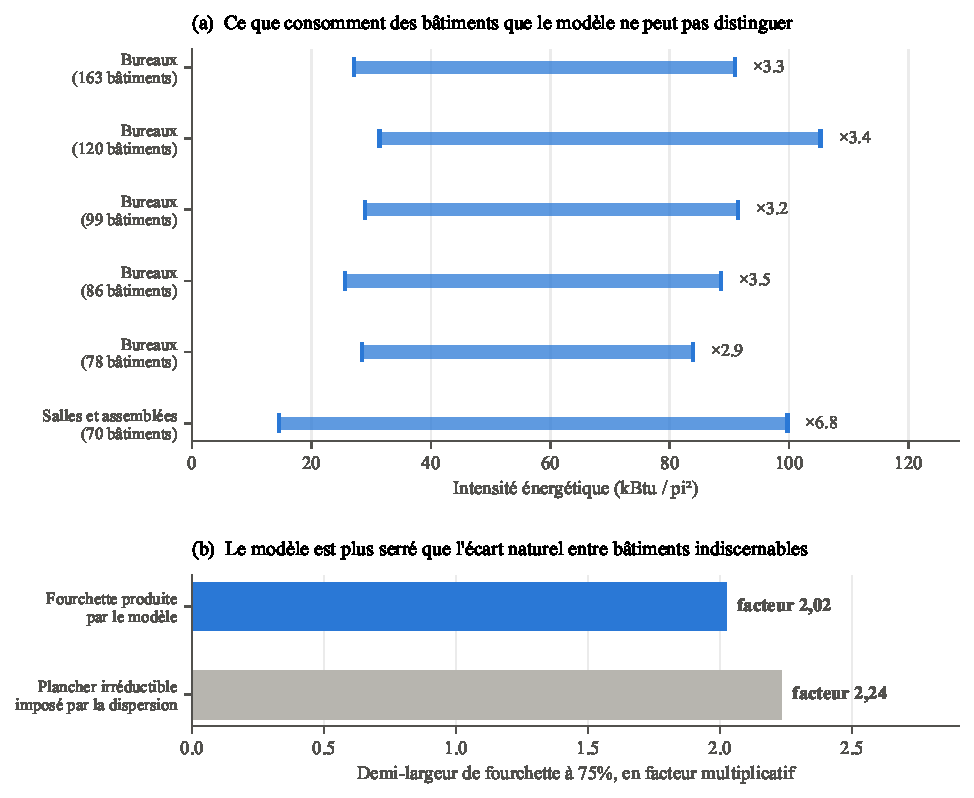
\includegraphics[width=\linewidth]{figures/plafond-performance.pdf}
\caption{En haut, l'étendue réelle des intensités au sein de groupes que le
modèle ne peut pas distinguer. En bas, la conséquence : la dispersion imposerait
à elle seule une fourchette d'un facteur 2,24, alors que le modèle en produit une
de 2,03.}
\end{figure}

\subsubsection*{L'explication physique}

Les variables disponibles décrivent \textbf{ce qu'un bâtiment est}, alors que sa
consommation dépend de \textbf{comment il est utilisé et exploité} :

\begin{itemize}[leftmargin=1.4em,itemsep=0.2em]
  \item le taux d'occupation et les horaires — un plateau à 30\,\% d'occupation
        contre un autre plein, ouvert 40~h ou 90~h par semaine : un facteur~2 à
        lui seul ;
  \item les équipements installés — salle serveurs, cuisine professionnelle,
        imagerie médicale : invisibles dans les données, décisifs dans la facture ;
  \item l'âge et le rendement des systèmes de chauffage et de climatisation ;
  \item la qualité de l'enveloppe — deux immeubles de 1960 dont l'un a été rénové
        sont indiscernables dans ce jeu de données ;
  \item les consignes de température et la régulation.
\end{itemize}

\subsection{Perspectives d'évolution}

\begin{constat}{La marge n'est pas dans l'algorithme}
Six familles de modèles se tiennent en quatre points de $R^2$, et le modèle de
fondation ne gagne que deux points. Investir dans un meilleur algorithme
reviendrait à optimiser la seule dimension qui ne bouge plus.
\end{constat}

Les gains sont dans les \textbf{données}, par ordre décroissant d'effet attendu :

\begin{enumerate}[leftmargin=1.6em,itemsep=0.2em]
  \item données d'occupation — effectifs, horaires d'ouverture ;
  \item inventaire des équipements énergivores ;
  \item âge et type des systèmes de chauffage et de climatisation ;
  \item indicateurs d'enveloppe — année de rénovation, performance thermique ;
  \item sous-comptage par usage.
\end{enumerate}

Deux extensions à moindre coût, indépendantes des données ci-dessus : exploiter
plusieurs millésimes plutôt qu'un seul, ce que le pipeline permet déjà ; et
mesurer l'empreinte de l'inférence, qui n'a pas été instrumentée alors que c'est
elle qui tourne en continu.

\subsection{Prochaines étapes recommandées}

\begin{table}[H]
\centering
\small
\begin{tabularx}{\linewidth}{@{}cXL{2.6cm}@{}}
\toprule
\textbf{Rang} & \textbf{Étape} & \textbf{Effort} \\
\midrule
1 & Confronter la priorisation à des audits réels — c'est le seul moyen de renseigner les indicateurs métier laissés vides & Externe au projet \\
2 & Rejouer le pipeline sur plusieurs millésimes et mesurer la stabilité des estimations dans le temps & Faible \\
3 & Instrumenter l'empreinte de l'inférence et la rapporter au nombre de bâtiments traités & Faible \\
4 & Négocier l'accès à une source d'occupation, même partielle, sur un sous-ensemble du parc & Élevé, hors périmètre technique \\
\bottomrule
\end{tabularx}
\caption{Étapes recommandées, par ordre de valeur.}
\end{table}

\subsection{Limites de la démarche}
\label{sec:limites-demarche}

Trois limites doivent accompagner la lecture de ce rapport.

\begin{description}[leftmargin=0em,style=nextline,itemsep=0.3em]
  \item[Les besoins sont reconstitués.] Aucune partie prenante n'a été
        interrogée. Les besoins ont été déduits de la documentation publique du
        programme et de la nature des données. Une collecte réelle aurait pu
        faire émerger des besoins que ce rapport ignore.
  \item[La garantie de couverture est marginale.] Elle vaut en moyenne sur un
        parc, pas bâtiment par bâtiment, et ne se transporte pas automatiquement
        à chaque typologie. C'est la limite principale de la méthode retenue, et
        elle est écrite dans l'interface.
  \item[Le rendu visuel de l'application n'a pas été vérifié automatiquement.]
        Les tests couvrent le comportement, pas l'apparence ; la vérification
        visuelle est restée manuelle.
\end{description}

\newpage
